\chapter{Q06}
\emph{Q6: Clear channel assessment (CCA) and low power listening (LPL) are the
two highlight features of BMAC. Explain how CCA and LPL work in BMAC?}

\section{B-MAC}
\subsection{Design goals of B-MAC}
\begin{itemize}
	\item Effective Collision Avoidance
	\item Simple Implementation, Small Code and RAM Size
	\item Efficient Channel Utilization
	\item Reconfigurable by Network Protocols
	\item Tolerant to Changing RF/Networking Conditions
	\item Scalable to Large Numbers of Nodes
\end{itemize}

\section{Clear Channel Assessment}

Take a signal strength sample when the channel is free - after a packaged is
transmitted

Samples are entered into a FIFO queue

Exponentially weighted moving average as a simple low pass filter.

Noise Floor estimation from RSSI

\subsubsection{Single-Sample Thresholding vs Outlier Detection}

\begin{center}
 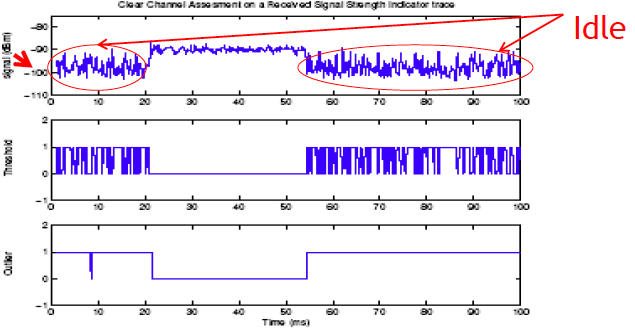
\includegraphics[scale=0.5]{img/CCA-RSSI.png}
\end{center}

\section{Low Power Listening}

Goal: minimize listening cost

Node periodically wakes up, turns radio on and checks channel

If activity -> stay awake

\begin{center}
 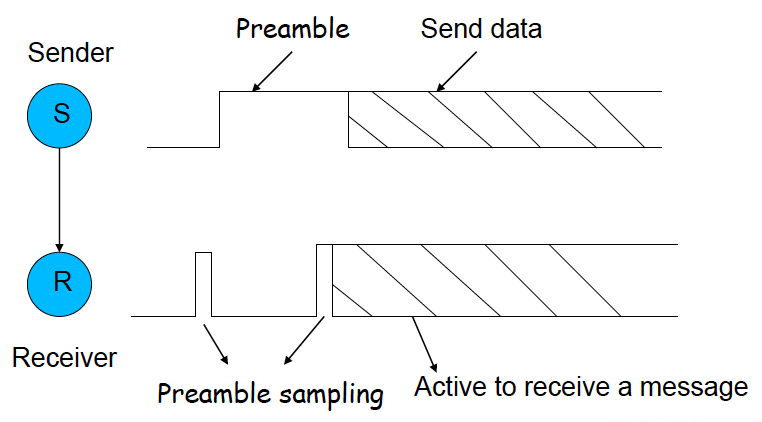
\includegraphics[scale=0.5]{img/LPL-PreambleSampling.png}
\end{center}

\subsection{Check interval}
\begin{description}
	\item[Too small] energy wasted on idle listening
	\item[Too large] energy wasted on transmissions (long preambles)
\end{description}

